\subsection{Fundamentals of Information Security}
It is important to understand what precisely is implied when discussing security. Therefore, we have to properly define it. For instance, the terms cybersecurity and information security are commonly used indistinguishably. The Cambridge Dictionary defines information security as \say{methods used to prevent electronic information from being illegally obtained or used}, and defines cybersecurity as \say{things that are done to protect a person, organization, or country and their computer information against crime or attacks carried out using the internet}. The definition for cybersecurity describes a much larger scope for security. 

Solms et al \cite{von_Solms_2013} supports this argument and reasons that information security is solely about securing the information, generally referred to as the asset, from potential threats posed by inherent vulnerabilities. Furthermore, they outlined that cybersecurity goes beyond protecting assets. Cybersecurity includes the insurance of those that operate in cyberspace in addition to any of their assets that can be achieved through cyberspace. Although the definition of information security and cybersecurity overlap each other, the latter is much more extensive in its definition. Overall, security is about securing assets against the most probable types of attacks, to the best ability \cite{andress2014the}.

Information security can be defined as the protection of information from potential abuse after various threats and vulnerabilities \cite{von_Solms_2013}. In a general sense, security means protecting our data and systems assets from whoever intends to misuse them. It includes several aspects of business, involving financial controls, human resources, and protection of the physical environment, as well as health and safety measures \cite{zinatullin2016the}. Security strives to secure ourselves against the most likely forms of attack, to the best ability.

Security is built on top of well-established principles like the Confidentiality, Integrity and, Availability (CIA) triad and the gold standard.

\subsubsection{The Confidentiality, Integrity, and Availability Triad}\label{subsec:cia}
Security can be complicated as discussed in Section \ref{sec:challenges-in-is}. Nonetheless, as described in Table \ref{fig:cia}, the CIA triad, provides a model to think about and discuss security concepts. It is commonly discussed in the information security literature \cite{andress2014the} \cite{srinivasan2016cissp} \cite{death2017information}. The CIA triad is commonly referred to as tenets of information security. Information assets that are tied to an application can be associated with a specified CIA requirement represented as a number or values suchlike, high, medium, or low, which can be determined through risk analysis \cite{srinivasan2016cissp}. 

\begin{figure}
    \centering
    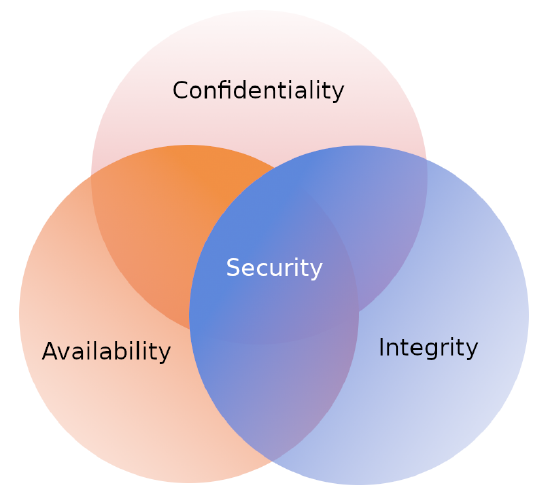
\includegraphics[width=0.5\textwidth]{chapter-2/cia-triad.png}
    \caption{The CIA Triad}\label{fig:cia}
\end{figure}

\paragraph{Confidentiality}
Confidentiality describes the capability to secure assets from parties that do not have the authorization to view them. 

\paragraph{Integrity}
The second concept describes the ability to prevent data from being changed in an unauthorized or undesirable manner. Integrity preserves the consistency of information both internally and externally.

\paragraph{Availability}
The final concept describes the ability to access data when required.

\subsubsection{The Gold Standard}

\paragraph{Authentication}
Identification is the claim of identity by a person, process, or other entity without implying the authenticity of the claim or privileges that could be affiliated with the identity. Many methods exist to claim our identity such as name abbreviations, fingerprints, portraits, and many more.

Authentication is the procedure used to validate whether the claim of identity is correct. A real-world example of authentication would be the usage of a username and password combination inside an application. Depending on the security level required of an asset, more factors can be used for the authentication mechanism, also known as multifactor authentication.

\paragraph{Authorization}
Besides claiming an identity and confirming the validity of that claim, we need to decide what the party is allowed to do and if access to specific resources is allowed or denied. 
% This can be accomplished through the concepts: authorization and access control.

\paragraph{Principle of least privilege}
An important authorization concept is the principle of least privilege. It mandates that only the bare minimum of access to a party should be allowed to function. As an example, a user account is only granted the access needed to perform their routine work. It is a very simple security measure that requires minimal effort, and it is highly effective.

\subparagraph{Access control}
At a high level, access control is about restricting access to a resource. Access control can be divided into two groups to either improve the design of physical security or cybersecurity. Generally, four basic actions can be performed: 
\begin{itemize}
    \item allowing
    \item access
    \item denying access
    \item limiting access
    \item revoking access
\end{itemize}
Most access control issues or situations can be described through these. Moreover, users that are not authorized should not be granted access. Therefore, it is best practice to disallow access by default.

Two main methods can be considered to implement access controls: access control lists (ACLs) and capabilities. ACLs often referred to as "ackles", are a very common choice of access control implementation. Typically, ACLs are implemented in the file systems on which our operating systems run and to control the flow of traffic in the networks to which our systems are connected. A capability-based approach to security uses tokens that manage our access. A good analogy would be the usage of a personal badge that grants access to certain doors inside a building. Notably, the right to access a resource is based completely on possession of the token, not who possesses it.

\paragraph{Auditing}
After going through the process of identification, authentication, and authorization, it is important to keep track of the activities that have occurred. Despite access being granted to the party, it is important that the party behaves according to the rules as it concerns security, ethics, business conduct, and so on. With an abundance of digital assets it has become a vital task to ensure that rules set forth are abided by.

\subsubsection{Cryptography}
Cryptography is the science of ensuring that assets are kept secure. The foremost security measure allowing cryptography is encryption, and often the terms are used interchangeably. Although in reality, encryption is a subset of cryptography. Encryption is the transformation of plaintext into ciphertext. 

Cryptology is not a recent invention. At the very least cryptology can be traced back as far as 2500 years and was considered an obscure science. It was well established with both ancient Greeks and Romans who practiced different forms of cryptography. A classic example of ancient cryptography is the Ceasar cipher as seen in Figure \ref{fig:ceasar-cipher}. After the fall of the Roman Empire, cryptology was flourishing in the Arabic world \cite{dooley2018history}.

\begin{figure}
    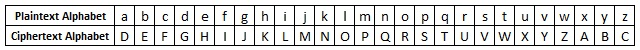
\includegraphics[width=0.5\textwidth]{chapter-2/ceasar-cipher.jpg}
    \caption{Ceasar Cipher}\label{fig:ceasar-cipher}
\end{figure}

Without cryptography, much of the internet-based activities we benefit from today would be at great risk. Cryptography is essential in computing, networking, and the great set of transactions that take place over such devices in everyday life. Cryptography has permitted us to become a very network-centric society. 
Data can be protected at rest, in motion, and to a certain extent, in use, because of cryptography. Thus allowing us to securely communicate and perform transactions when sensitive data is involved.

The process of encrypting plaintext and decrypting ciphertext is described as a cryptographic algorithm. To either encrypt or decrypt a message, cryptographic algorithms commonly use a key, or multiple keys, with a range of possible values for the key referred to as the keyspace. The harder the keyspace, the harder it is to decrypt the message. We will take a brief look at some popular cryptographic algorithms.

\subsection{Symmetric cryptography}
Symmetric cryptography, also referred to as private key cryptography, utilizes a single key for both encryption of the plaintext and the decryption of the ciphertext as can be seen in Figure \ref{fig:sym-crypt}. A symmetric cipher only works if both the sender and the receiver own same key to unlock the cipher. Therefore, everyone who uses a symmetric cipher must have the same set of keys and must use them in the correct order \cite{dooley2018history}.

\subsection{Asymmetric cryptography}
When a different key is used for encryption and decryption, we have an asymmetric system in place. Asymmetric cryptography can also be referred to as public key cryptography. Asymmetric cryptography relies on a public key to encrypt data from the sender, and a private key to decrypt data that arrives at the receiving end as seen in Figure \ref{fig:asym-crypt}. Due to the mathematical complexity of the operations to create the private and public keys, no method exists at present to reverse the private key from the public key.

\subsection{Hash functions}
Unlike both symmetric and asymmetric cryptography, which relies on keys for encryption and decryption, some algorithms do not require keys, known as hash functions. Hash functions generate a generally unique and fixed-length hash value, referred to as a hash, based on the original message as seen in Figure \ref{fig:hash}. Any form of change to the message will change the hash as well. Furthermore, hash functions do not allow for the contents of the message to be read, though they can be utilized to determine the confidentiality of the message. Some hash algorithms i0.5nclude Message-Digest 5 (MD5), MD2, MD4, SHA-2, and RACE. 

\paragraph{Digital signatures}
A good example of where hash functions are utilized is digital signatures. To detect any changes to the content of the message, digital signatures make it possible to sign a message to ensure the authenticity from the sending party. This is accomplished by generating a hash of the message, and then using the senders private key to encrypt the hash, thereby creating a digital signature. The receiving party can use the senders public key to decrypt the digital signature, thereby restoring the original hash of the message.

Digital signatures are now recognized as legally binding in many countries, allowing them to be used for certifying contracts or notarizing documents, for authentication of individuals or corporations, as well as components of more complex protocols. Broadly speaking, a digital signature is analogous to a handwritten signature, which provides much stronger security guarantees \cite{katz2010digital}. 

\subparagraph{Certificates}
Another form of cryptography for message signing is the usage of digital certificates, commonly known as certificates. Certificates link together a public key and an individual, typically by taking the public key and something to identify the individual, suchlike a name and address, and having them signed by a certificate authority (CA). A CA is a trusted entity that is responsible for digital certificates. The advantage of using a certificate is that it verifies that a public key is associated with a particular individual.

\subsection{Software Engineering}
Software is embedded into today's society, and it ranges from simple embedded systems to complex, worldwide information systems. There is no natural limit to the potential of software. However, because of this freedom, software can easily become highly complex, difficult to comprehend, and costly to change. Individual approaches to software development did not scale up to large and complex software systems. Thus, the notion of software engineering was proposed in 1968. Software engineering aims to assist professional software development rather than individual programming. It is an engineering principle concerned with all aspects for the creation of software \cite{book:se_sommervile_2021}.

The SLDC is a process with related activities that leads to the production of a software system. In this section, the SDLC is presented and what common security vulnerabilities are found in deployed software. Lastly, the role of security in the SDLC is discussed. 

\subsubsection{The Software Development Life Cycle}
The purpose of the SDLC has adjusted over time since the first concept was presented by Herbert Benington in 1956. Initially, the concept of the SDLC was about understanding what needed to be done. Later, \textit{sequential} SDLC models were introduced and had strongly controlled development activities. The growing focus on processes, strong control, tool support and so forth led to a countermovement advocating for self-organization, iterative life cycles and suchlike. As a result, \textit{agile} methodologies and the parallel plan-driven and the agile cultures grew in importance. Today, it is understood that both the sequential and agile approach to software development have their pros and cons \cite{Kneuper_2017}. Though a variety of SDLC models exist, an overview of the SDLC phases is shown in figure \ref{fig:sdlc-phaces}.

\begin{figure}
    \centering
    \caption{The SDLC phases}
    \label{fig:sdlc-phaces}
    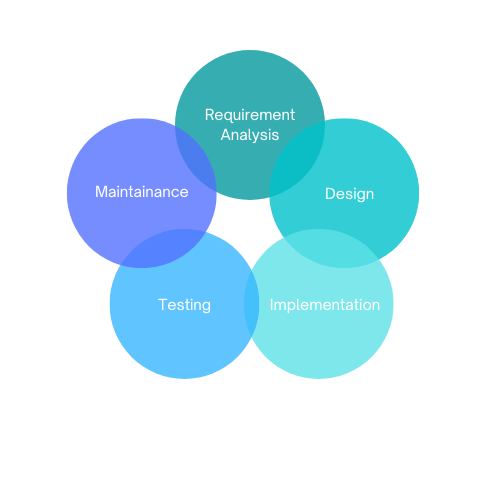
\includegraphics[width=0.5\textwidth]{chapter-2/sdlc-phases}
\end{figure}

\subsection{Software Security Awareness and Security Standards}
Today's software demands the highest security standard from companies and developers. Although many security standards exist, this thesis will cover the ones most relevant to the study. These include standards such as the National Institute of Standards and Technology (NIST),lists such as the Common Weakness Enumeration (CWE) and projects from OWASP such as the OWASP Top 10, OWASP ASVS, and the OWASP MASVS. 

\subsubsection{The Open Web Application Security Project}
OWASP is a leader in software security. As a non-profit organization focusing on the improvement of software security, it has become a source for security tools, resources, education and training. Furthermore, it has a worldwide community of software security professionals. Security awareness documents such as the OWASP Top 10 and standards such as the ASVS and MASVS are part of OWASP as well is SKF.

\subsubsection{The Top 10}\label{sec:owasp-top-10}
The OWASP Top 10 is a regularly updated security awareness document concerning web applications, focusing on the ten most critical risks. Each security risk has a list of mapped CWEs. Table \ref{} describes the top ten security risks by OWASP Top 10. Although the document exist to bring awareness, it has not stopped companies to use it as a standard to secure software. The OWASP Top 10 provides some recommendations on how to use it as a standard. Additionally, it provides ways to prevent the common attacks. However, it is still encourages to use a real standard such as the ASVS.

\begin{table}
    \centering
    \caption{The OWASP Top 10 as of 2021}
    \label{tab:owasp-top-ten}
    \begin{tabulary}{1.0\textwidth}{|l|L|}
        \hline
        \textbf{ID} & \textbf{Description} \\
        \hline
        AO1:2021 & Broken Access Control \\
        \hline
        AO2:2021 & Cryptographic Failures \\
        \hline
        AO3:2021 & Injection \\
        \hline
        AO4:2021 & Insecure Design \\
        \hline
        AO5:2021 & Security Misconfiguration \\
        \hline
        AO6:2021 & Vulnerable and Outdated Components \\
        \hline
        AO7:2021 & Identification and Authentication Failures \\
        \hline
        AO8:2021 & Software and Data Integrity Failures \\
        \hline
        A09:2021 & Security and Logging and Monitoring Failures \\
        \hline
        A10:2021 & Server-side Request Forgery (SSRF) \\
        \hline 
    \end{tabulary}
\end{table}

\paragraph{Broken Access Control}
Implementing a reliable access control mechanism is often underestimated by developers, causing unauthorized access to application content and functions.

\paragraph{Cryptographic Failures}
Data such as passwords, credit cards numbers, health records, personal information, and business secrets require extra protection. Therefore, it is important to determine how much protection data needs in transit and at rest. When encryption is implemented poorly, attackers can retrieve data in its unencrypted state.

\paragraph{Injection}
Injection attacks include SQL, NoSQL, OS command, Object Relational Mapping (ORM), LDAP, and Expression Language (EL) or Object Graph Navigation Library (OGNL) injections. Injection vulnerabilites are introduces when:

\begin{itemize}
    \item User entered data is not validated, filtered or sanitized
    \item Dynamic queries or non paratemetized calls without context-aware escaping are used directly in the interpreter.
    \item Hostile data is used within ORM search parameters to extract additional, sensitive records.
    \item Hostile data is directly used or concatenated. The SQL or command contains the structure and malicious data in dynamic queries, commands, or stored procedures.
\end{itemize}

\paragraph{Insecure Design}
Business often fail to determine what level of security design is required, due to a lack of business risk profiling to the software being developed. As a result, software is insecure by design. It is therefore important to include security into the SDLC and ensure security activities are performed from the beginning.

\paragraph{Security Misconfiguration}
Security misconfigurations are security controls that are configured improperly of left insecure, putting assets at risk. These include configuration such as default accounts and password that are not changed, unnecessary features that are enabled, outdated software and many more. Without proper security in place, systems are at more risk.

\paragraph{Vulnerable and Outdated Components}
Software often rely on third party components on both the server-side and client-side. Unfortunately, these components may have software vulnerabilities when they are developed at high speed without doing any security tests before publishing.

\paragraph{Identification and Authentication Failures}
Vulnerabilities in authentication schemes can lead to serious and damaging data breaches. Therefore, developers need to ensure that the user's identity, authentication, and session management is properly confirmed.

\paragraph{Software and Data Integrity Failures}
Moderns software architecture has become more and more complex. As a result applications often rely on plugins, libraries, or modules from untrusted sources, repositories and content delivery networks. Critical data and software updates are often added to the delivery pipeline without verifying their integrity resulting and software data integrity failures \cite{site:A08_2022}.

\paragraph{Security Logging and Monitoring Failures}
The ninth category in the OWASP Top 10 cover security logging and monitoring. Loggin and monitoring provides raw data that assists in identifying possible security threats. This category is difficult to test for since it often involves interviewing or asking if attacks were found during a penetration test. The category exist because without logging and monitoring, breaches simply cannot be detected.

\paragraph{Server Side Request Forgery}
Server Side Request Forgery (SSRF) happen when an attacker can abuse the functionality of the server to read or update internal resources.

\subsubsection{The Application Security Verification Standard}
The ASVS is a security standard that provides developers a list of security requirements for secure development. The standard can be used to establish a level of confidence in security of web applications. The requirements are categorized in 14 categories that are described in table \ref{tab:asvs-categories}. Each ASVS category has its objective and set of security requirements. Furthermore, the ASVS divides the risk severity into three levels. It is up to the organization or development team to decide what security requirements must be implemented. This can be done in the early phases of the SDLC during planning and the requirements' analysis phase.

\begin{table}
    \centering
    \caption{ASVS Categories}
    \label{tab:asvs-categories}
    \begin{tabulary}{1.0\textwidth}{|l|L|}
        \hline
        \textbf{ID} & \texbf{Category} \\                                                    
        \hline
        \textbf{V1} & Architecture, Design, and Threat Modeling \\
        \hline
        \textbf{V2} & Authentication \\
        \hline
        \textbf{V3} & Session Management \\
        \hline
        \textbf{V4} & Access Controll \\
        \hline
        \textbf{V5} & Validation, Sanitization and Encoding \\
        \hline
        \textbf{V6} & Stored Cryptography \\
        \hline
        \textbf{V7} & Error Handling and Logging \\
        \hline
        \textbf{V8} & Data Protection \\
        \hline
        \textbf{V9} & Communication \\
        \hline
        \textbf{V10} & Malicious Code \\
        \hline
        \textbf{V11} & Business Logic \\
        \hline
        \textbf{V12} & Files and Resources \\
        \hline
        \textbf{V13} & API and Web Service \\
        \hline
        \textbf{V14} & Configuration \\
        \hline
    \end{tabulary}
\end{table}


\paragraph{ASVS Level 1}
Applications achieve Level 1 if it sufficiently defends against security vulnerabilities that are easy to discover, and are included in the OWASP Top 10. Level 1 is the bare minimum that all applications should strive when implementing security. Furthermore, Level 1 security requirements can be tested against automatically by tools.

\paragraph{ASVS Level 2}
Applications achieve Level 2 - or standard - if it sufficiently defends against most the of security risks that are associated with today's software. It guarantees that security controls are in place, effective, and used within the application. Level 2 applications include applications that handle significant business-to-business transactions, such as healthcare information, implement critical business or sensitive functions, or other sensitive assets.

\paragraph{ASVS Level 3}
The highest verification level is the ASVS Level 3. Level 3 applications are commonly reserved for application that require a substantial levels of security verification, such as applications that are developed for the military, health and safety, critical infrastructure, and so on.

\subsubsection{The Mobile Application Security Verification Standard}
The MASVS is a security standard similar to the ASVS, but offers a security standard for mobile applications specifically. Closely related to the MASVS is the MSTG, which offers test cases against the security requirements defined in the MASVS. Like the ASVS, the security requirements defined in the MASVS are devided into different categories that are described in table \ref{tab:masvs-categories}. As seen, the MASVS has lesser categories compared with the ASVS, and also focuses a lot more on how mobile applications handle, store and protect sensitive data. As with the ASVS, which security requirements to implement needs to be decided during the planning and requirements analysis phase of the SDLC by the team responsible for the development of the application.

The MASVS defines two verification levels, MASVS-L1 and MASVS-L2. Additionally, it adds a set of \emph{reverse engineering resiliency requirements}, MASVS-R.

\paragraph{MASVS Level 1: Standard Security}
The MASVS-L1 is the standard security level all mobile applications should adhere to. Implementing MASVS-L1 ensures that basic security requirements in terms of code quality, handling of sensitive data, and interaction with the mobile environment is fulfilled. Testing must be done to verify wether the security controls are implemented correctly.

\paragraph{MASVS Level 2: Defense-in-Depth}
Going beyond the standard security requirements introduces mobile applications to MASVS-L2. A threat model has be in place to achieve MASVS-L2. Mobile apps such as banking apps have to adhere to MASVS-L2.

\paragraph{Resiliency Against Reverse Engineering and Tampering}
The MASVS-R protects mobile applications against client side attacks such as tampering, modding, or reverse engineering to extract sensitive code or data. The MASVS-R may be applied to applications handle highly sensitive data to protect its intellectual property or tamper-proofing an app.

\begin{table}
    \centering
    \caption{MASVS categories}
    \label{tab:masvs-categories}
    \begin{tabulary}{1.0\textwidth}{|L|L|}
        \hline
        \textbf{ID} & \textbf{Category} \\
        \hline
        \textbf{V1} & Architecture, Design and Threat Modeling \\
        \hline
        \textbf{V2} & Data Storage and Privacy Requirements \\
        \hline
        \textbf{V3} & Cryptography Requirements \\
        \hline
        \textbf{V4} & Authentication and Session Management \\
        \hline
        \textbf{V5} & Network Communication Requirements \\
        \hline
        \textbf{V6} & Platform Interaction Requirements \\
        \hline
        \textbf{V7} & Code Quality and Build Settings Requirements \\
        \hline
        \textbf{V8} & Resilience Requirements \\
        \hline
    \end{tabulary}
\end{table}


